\newpage
\hypertarget{stringRep vis}{}
\subsection{Implementing stringRep}
\visHeader

\begin{itemize}

\item[$\blacktriangleright$] Visual SDMs support arbitrary nesting of \emph{for each} story nodes via special guards. In \hyperlink{emptyPartition vis}{Section
5.1} we used the \texttt{[end]} edge guard to terminate a loop. Now we'll use a new guard, the \texttt{[each time]}\define{[each time]} guard, to indicate control flow that is \emph{nested} and
executed for each match. Go ahead and create the SDM for \texttt{Box::toString} until it closely resembles Fig.~\ref{fig:sdm_tostring_1}. 

\vspace{0.5cm}

\begin{figure}[htbp]
\begin{center}
  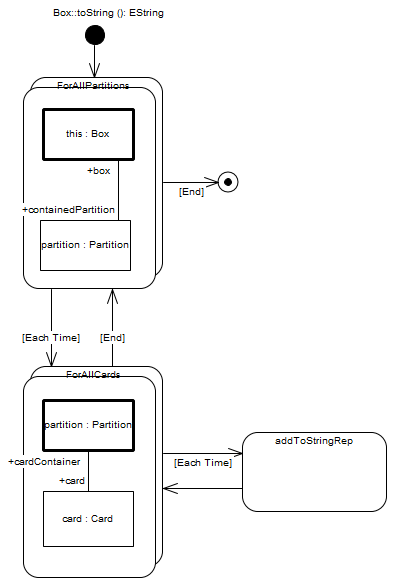
\includegraphics[width=0.8\textwidth]{ea_toStringStart}
  \caption{Control flow with nested loops} 
  \label{fig:sdm_tostring_1}
\end{center}
\end{figure}

\clearpage

\item[$\blacktriangleright$] Knowing \texttt{addToStringRep}'s default node type will not allow it to invoke our helper method, change it
into a \texttt{StatementNode}. Then, analogously to how you established a \emph{MethodCallExpression} for \texttt{grow}, have this node invoke
\texttt{this.addToStringRep(Card)}. 

\vspace{0.5cm}

\item[$\blacktriangleright$] You can see in the \texttt{Source} statement that a \texttt{Card} parameter is required. Update the \texttt{Parameter Values}
field to include \texttt{card} so we may pass the object variable to the method. Although you can simply type in \texttt{card}, the best practice is to
double-click the field to pop-up a new dialogue. This way, complex expressions can be constructed by repeatedly double-clicking the fields.

\vspace{0.5cm}

\begin{figure}[htbp]
\begin{center}
  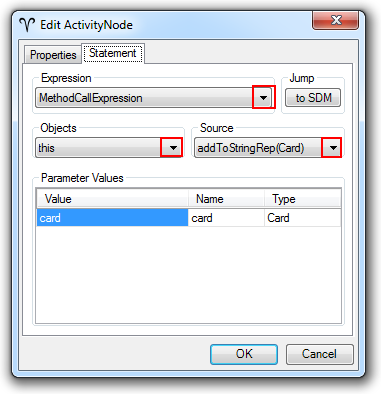
\includegraphics[width=0.5\textwidth]{ea_editStatementNode}
  \caption{Add a parameter to the \emph{MethodCallExpression}}
  \label{fig:editStatement}
\end{center}
\end{figure}

\item[$\blacktriangleright$] To complete the SDM, return the final string representation value of the box via an \emph{AttributeValueExpression} in
the stop node (Fig.~\ref{fig:toStringStopNode}).\define{AttributeValue\-Expression}This is a new expression type we haven't encountered before. It simply
updates and binds the return \texttt{stringRep} attribute to the whatever value with the same name was edited in each invocation of
\texttt{add\-To\-String\-Rep}.

\newpage

\begin{figure}[htbp]
\begin{center}
  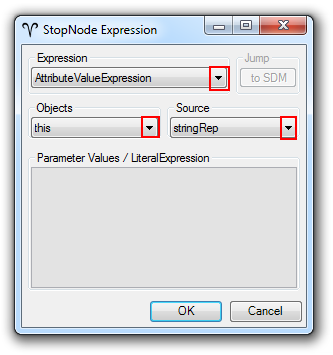
\includegraphics[width=0.5\textwidth]{ea_returnAttributeStopNode}
  \caption{Specify a return value}
  \label{fig:toStringStopNode}
\end{center}
\end{figure}

\vspace{0.5cm}

\item[$\blacktriangleright$] Take some time to compare and reflect on the complete SDM as depicted in Fig.~\ref{fig:sdm_tostring_5}.  The idea was to abstract
from the actual text representation of the box and model the necessary traversal of the data structure. The helper method \texttt{addToStringRep} could, for
example, build up a string buffer and update this string representation. 

\vspace{0.5cm}

\item[$\blacktriangleright$] While modelling this SDM, we have seen that \emph{for each} story nodes can be nested, and have learnt two new uses of
\emph{MethodCallExpressions} that provide a type safe means of invoking methods from SDMs.

\vspace{0.5cm}

\item[$\blacktriangleright$] As always, save, validate, and build your metamodel in Eclipse. To see how this is done in the
textual syntax, check out the nested loops in Fig.~\ref{fig:toStringFlow} and each pattern in Fig.~\ref{fig:toStringPatterns}.

\newpage

\vspace*{2cm}

\begin{figure}[htbp]
\begin{center}
  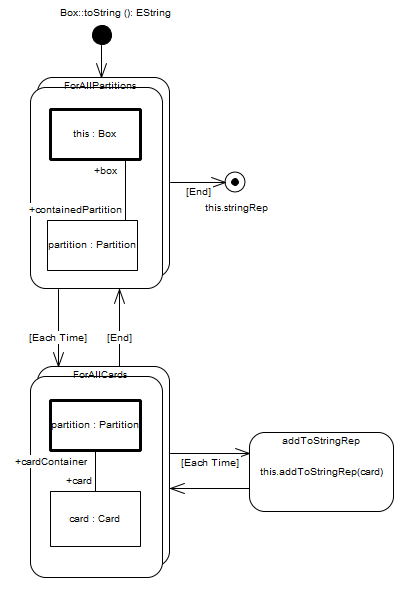
\includegraphics[width=0.8\textwidth]{ea_toStringComplete}
  \caption{The complete SDM for \texttt{Box::toString}}  
  \label{fig:sdm_tostring_5}
\end{center}
\end{figure}
\FloatBarrier

\jumpSingle{sec:fastCard}

\end{itemize}
